\documentclass[x11names]{beamer}
\usepackage{etex,beamerfoils}
\usepackage{array,pifont,amsmath,latexsym,epsfig,amsfonts,yfonts}
\usepackage{amstext,amsopn,amsxtra,amsgen,amsbsy,amscd,amssymb,dcolumn,graphicx,setspace,pgfplots,booktabs,natbib}
\usepackage[normalem]{ulem}
\usepackage[all]{xy}
\beamertemplatetheoremsnumbered
\setbeamertemplate{caption}[numbered]
\usetheme{Copenhagen}
\definecolor{NewBlue}{RGB}{4, 114, 155}
\definecolor{magenta}{cmyk}{0,1,0,0}
\usecolortheme[named=NewBlue]{structure}
%\usecolortheme[named=SkyBlue4]{structure}

\newcommand{\D}{\displaystyle}
\newcommand{\E}{\begin{eqnarray*}}
\newcommand{\F}{\end{eqnarray*}}
\newcommand{\EE}{\begin{eqnarray}}
\newcommand{\FF}{\end{eqnarray}}
\newcommand{\IZ}{\begin{itemize}}
\newcommand{\ZI}{\end{itemize}}
\newcommand{\EN}{\begin{enumerate}}
\newcommand{\NE}{\end{enumerate}}
\newcommand{\itemc}{\item[$\circ$]}
\newcommand{\IZdash}{\begin{itemize} \renewcommand{\labelitemi}{-}}
\newcommand{\tn}{\textnormal}

% New commands to assist Beamer
\newcommand{\itemi}{\item<1->}
\newcommand{\itemii}{\item<2->}
\newcommand{\itemiii}{\item<3->}
\newcommand{\itemiv}{\item<4->}
\newcommand{\itemv}{\item<5->}
\newcommand{\itemvi}{\item<6->}
\newcommand{\itemvii}{\item<7->}
\newcommand{\itemviii}{\item<8->}
\newcommand{\itemix}{\item<9->}
\newcommand{\itemx}{\item<10->}

\newcommand{\itemci}{\item[$\circ$]<1->}
\newcommand{\itemcii}{\item[$\circ$]<2->}
\newcommand{\itemciii}{\item[$\circ$]<3->}
\newcommand{\itemciv}{\item[$\circ$]<4->}
\newcommand{\itemcv}{\item[$\circ$]<5->}
\newcommand{\itemcvi}{\item[$\circ$]<6->}
\newcommand{\itemcvii}{\item[$\circ$]<7->}
\newcommand{\itemcviii}{\item[$\circ$]<8->}
\newcommand{\itemcix}{\item[$\circ$]<9->}
\newcommand{\itemcx}{\item[$\circ$]<10->}


\newcommand{\fr}{\frame}
\newcommand{\ft}{\frametitle}
\newcommand{\ons}{\onslide}
\newcommand{\tc}{\textcolor}

\pgfplotsset{height =7cm,compat=1.7,width=7cm,
    standard/.style={
    	unit vector ratio*=1 1 1,
        axis x line=middle,
        axis y line=middle,
        enlarge x limits=0.15,
        enlarge y limits=0.15,
        every axis x label/.style={at={(current axis.right of origin)},anchor=north west},
        every axis y label/.style={at={(current axis.above origin)},anchor=north east}
    }
}
\newcommand{\drawge}{-- (rel axis cs:1,0) -- (rel axis cs:1,1) -- (rel axis cs:0,1) \closedcycle}
\newcommand{\drawle}{-- (rel axis cs:1,1) -- (rel axis cs:1,0) -- (rel axis cs:0,0) \closedcycle}

\usetikzlibrary{patterns}
\usetikzlibrary{arrows}
\usetikzlibrary{shapes}

\renewcommand{\bibsection}{}

% Watermark example: https://texblog.org/2012/02/17/watermarks-draft-review-approved-confidential/
\usepackage{draftwatermark}
\SetWatermarkText{This content is protected and may not be shared uploaded or distributed.}
\SetWatermarkScale{0.25}
\SetWatermarkAngle{0}
\SetWatermarkColor[gray]{1.0}
\setbeamercolor{background canvas}{bg=}%transparent canvas

\title[Business Cycle Data\hspace{2em}\insertframenumber/
\inserttotalframenumber]{Introduction to Business Cycle Data}
\author{Brian C.~Jenkins \\ ~ \\University of California, Irvine}

\begin{document}

\frame{\maketitle}


\fr{
\ft{Business Cycle Data}

\IZ
\itemi The \emph{business cycle} is the fluctuation of many macroeconomic quantities that last for about 1.5 to 8 years.

\

\itemii Business cycle fluctuations are costly:

	\IZ
	\itemiii Misallocations of capital and labor. 
	\itemiv Particularly painful for workers that become unemployed and for the families of workers who become unemployed.
	\ZI
	
\ZI


}


\fr{
\ft{Business Cycle Data}

\IZ
\item We will examine two historically-competing schools of thought:

	\EN
	\itemii \textbf{Real Business Cycle (RBC)} theory: fluctuations in real quantities are primarily due to TFP shocks; i.e., shocks to the production function.
	\itemiii \textbf{New-Keynesian (NK)} theory: fluctuations are largely driven by aggregate demand and affect real quantities because of nominal rigidities (e.g., sticky prices).
	\NE
	
\

\itemiv Both approaches have merits and shortcomings and elements of both are integrated into contemporary business cycle theory.
\ZI
}

\fr{
\begin{figure}[h] \caption{\label{fig_009_rbc_aggregate_data} \textbf{GDP, consumption, investment, and hours} for the US from January 1948 to April 2022. {\tiny Source: FRED}.}
\begin{center}\hspace*{-.5cm}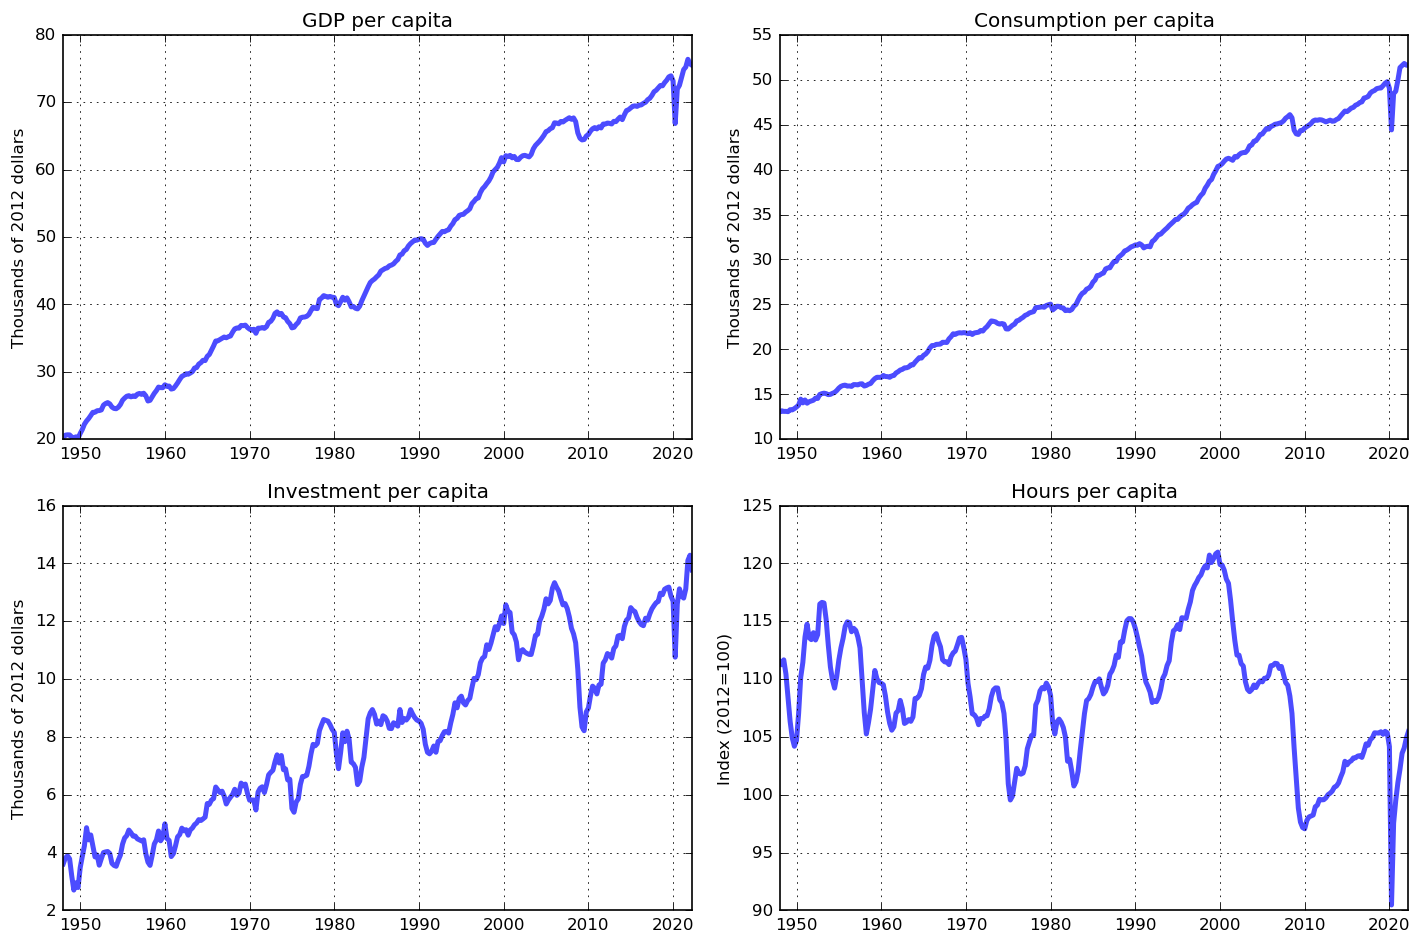
\includegraphics[height = 7.cm]{fig_009_rbc_aggregate_data.png}\end{center}
\end{figure}
}


\fr{
\ft{Trend and Cycle Components}

\IZ
\itemi Suppose that the value of a time series process $X_t$ can be decomposed into two components: a \emph{trend} component and 
a \emph{cyclical} component.

    \EE
    X_t & = & X_t^{trend} + X_t^{cycle}
    \FF

\

\itemii The trend component is the long-run path about which the series fluctuates.

\

\itemiii The cyclical component is the difference between the value of a time series and the trend:


	\EE
	X_t^{cycle} & = & X_t - X_t^{trend}
	\FF
\ZI

%\itemii 

}


\fr{
\ft{Trend and Cycle Components}

\IZ
\itemi Often, it's useful to express the cyclical component of a time series as the percent deviation of the series from trend (divided by 100):

\EE
\hat{x}_t & = \frac{X_t-X_t^{trend}}{X_t^{trend}} = \frac{X_t^{cycle}}{X_t^{trend}}
\FF
	
\

\itemii Note:

\EE
\frac{X_t-X_t^{trend}}{X_t^{trend}} = \frac{X_t^{cycle}}{X_t^{trend}} & \approx \log X_t - \log X_t^{trend}
\FF

\ZI

}


\fr{
\ft{Trend and Cycle Components}
\begin{exampleblock}{Example: Percent Deviation from Trend}

\IZ
\itemi Suppose:
	\EE
	X_t & = & 220\\
	\pause X^{trend}_t & = & 215
	\FF
	
\itemiii Then:
	\EE
	\pause \frac{X_t-X^{trend}_t}{X^{trend}_t} & = & \frac{220-215}{215} \, = \, 0.0233
	\FF
	\pause and:
	\EE
\log X_t - \log X^{trend}_t & = & \log 220-\log 215 \, = \, 0.0230
	\FF

\ZI
\end{exampleblock}
}

\fr{
\begin{figure}[h] \caption{\label{fig_009_rbc_gdp_actual_trend} \textbf{GDP, consumption, investment, and hours} per capita for the US from January 1948 to April 2022. {\tiny Source: FRED}.}
\begin{center}\hspace*{-.5cm}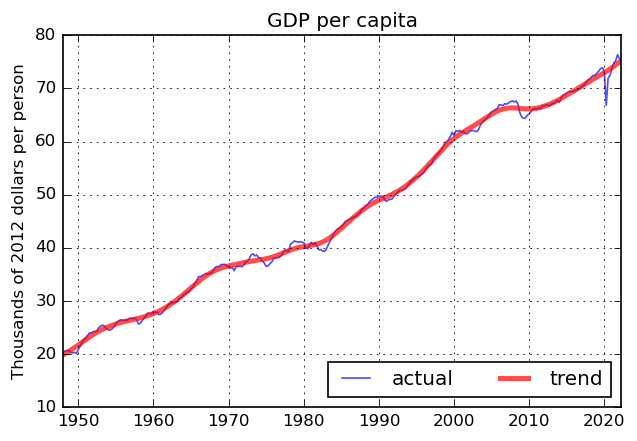
\includegraphics[height = 7.cm]{fig_009_rbc_gdp_actual_trend.png}\end{center}
\end{figure}
}

\fr{
\begin{figure}[h] \caption{\label{fig_009_rbc_gdp_aggregate_and_cyclical_data} \textbf{US GDP per capita:} actual, trend, and cycle from January 1948 to April 2022. {\tiny Source: FRED}.}
\begin{center}\hspace*{-.5cm}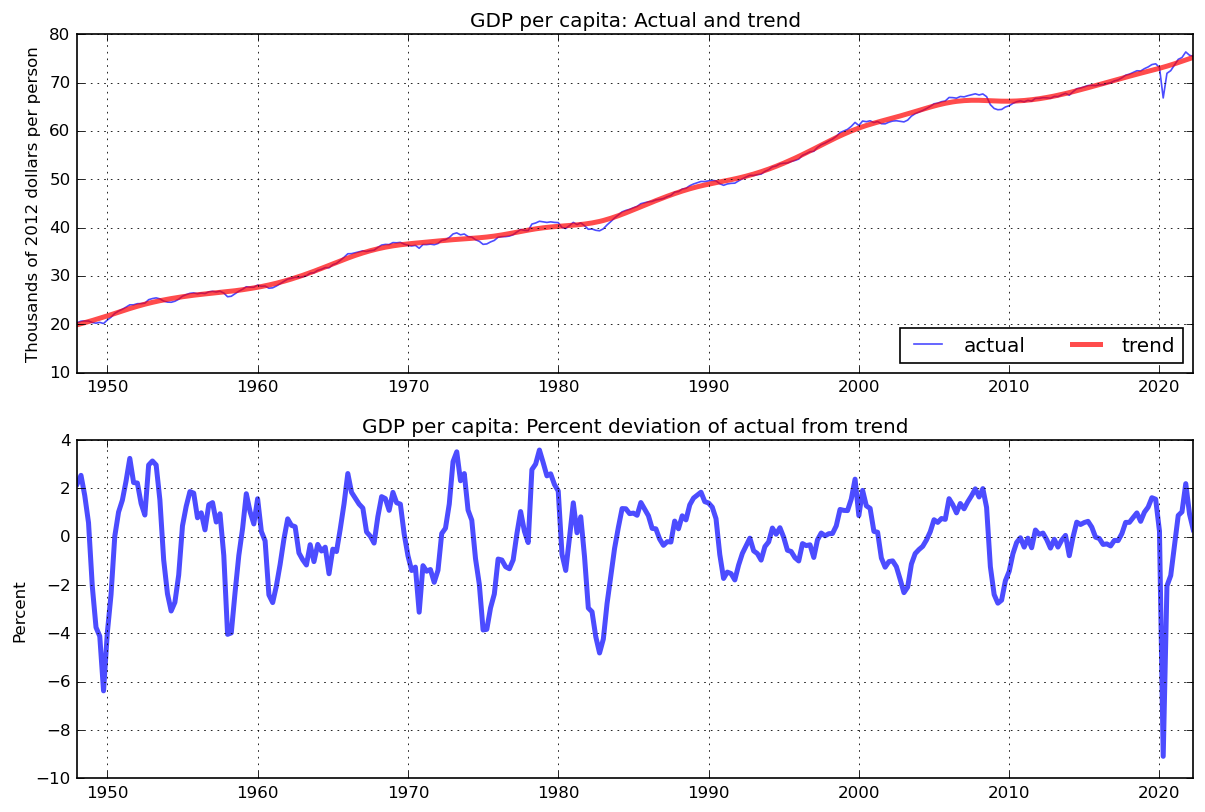
\includegraphics[height = 7.cm]{fig_009_rbc_gdp_aggregate_and_cyclical_data.png}\end{center}
\end{figure}
}

\fr{
\begin{figure}[h] \caption{\label{fig_009_rbc_all_cyclical_data} \textbf{Business cycle components of GDP, consumption, investment, and hours} for the US from January 1948 to April 2022. {\tiny Source: FRED}.}
\begin{center}\hspace*{-.5cm}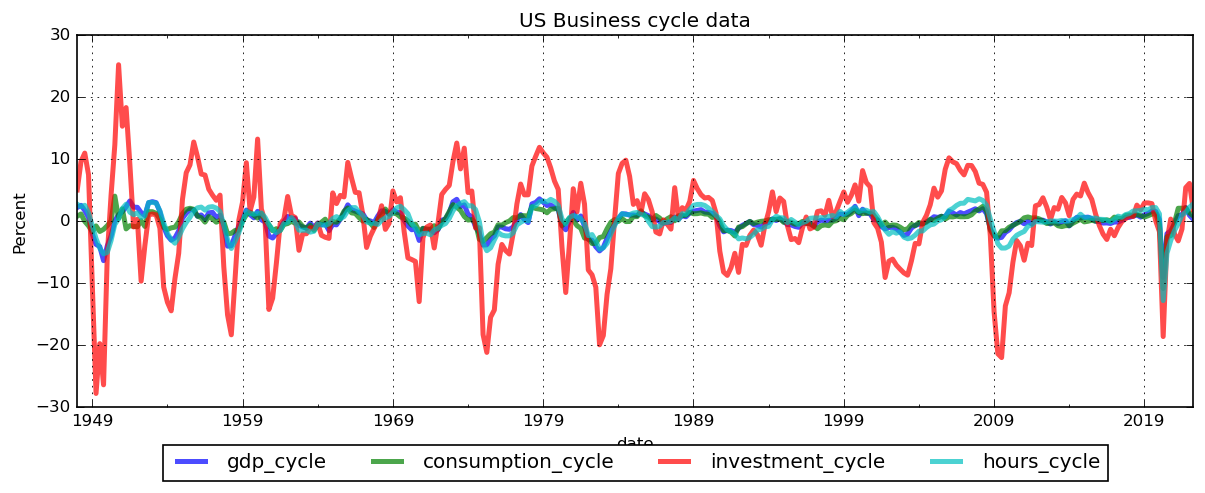
\includegraphics[height = 4.5cm]{fig_009_rbc_all_cyclical_data.png}\end{center}
\end{figure}
}

\fr{
\begin{table}[h] \caption{\label{tab009_rbc_data_std_devs} \textbf{Standard deviations of real business cycle data} from January 1948 to April 2022. Units are percent deviations from trend. {\tiny Source: FRED}.}
\begin{center}\hspace*{-.5cm}

\begin{tabular}{lr}
\toprule
GDP         &  1.688 \\
Consumption &  1.337 \\
Investment  &  7.400 \\
Hours       &  2.063 \\
\bottomrule
\end{tabular}
\end{center}
\end{table}
}

\fr{
\begin{table}[h] \caption{\label{tab009_rbc_data_correlations} \textbf{Correlations of real business cycle data} from January 1948 to April 2022. Units are percent deviations from trend. {\tiny Source: FRED}.}
\begin{center}\hspace*{-.5cm}

\begin{tabular}{lrrrr}
\toprule
{} &    GDP &  Consumption &  Investment &  Hours \\
\midrule
GDP         &  1.000 &        0.814 &       0.836 &  0.884 \\
Consumption &  0.814 &        1.000 &       0.645 &  0.757 \\
Investment  &  0.836 &        0.645 &       1.000 &  0.764 \\
Hours       &  0.884 &        0.757 &       0.764 &  1.000 \\
\bottomrule
\end{tabular}
\end{center}
\end{table}
}




\end{document}